\documentclass[twocolumn,10pt]{article}
\usepackage[utf8]{inputenc}

\usepackage{lipsum}
\usepackage[top=1in, bottom=1in, left=1in, right=1in]{geometry}
\usepackage[numbers]{natbib}


\usepackage[pdftex]{graphicx}
% declare the path(s) where your graphic files are
\graphicspath{{./img/}}

\title{State-based Markov Feature Learning for Gas Turbine Anomalies}
\author{Thurston Sexton \& Connor Armstrong}
\date{December 15, 2017}

\begin{document}
\maketitle

\section{Introduction}

Gas turbines are the beating hearts of modern industry, by converting a variety of fuels to electrical current they are capable of producing up to 225 MW of power. These incredibly complicated systems are vital to the function of factories and homes, meaning any unscheduled downtime is unacceptable. Traditionally, the most popular way to identify turbine anomalies is monitoring exhaust gas temperatures (EGTs) exiting combustion chambers. Traditional approaches are reliant upon rigid handcrafted features derived from prior engineering knowledge. Knowledge-based features are hindered by poor predictive performance, and crafting "good" features is an extremely time-consuming manual process. Improving the versatility and accuracy of anomaly detection requires a feature learning solution capable of autonomously creating efficient features from raw data. 

\subsection{Existing literature}
%List any major feature learning and/or prediction approaches out there that might specifically apply to sensor/turbine anomaly prediction. We want to end up talking about the methodology in \citep{gas_turbine} and how we're extending it. e.g: 

Previous studies on anomaly detection in gas turbines have investigated the effectiveness of supervised and unsupervised prediction methods on fixed data sets; however feature learning is rarely discussed \cite{yan2015}. 

A prior gas turbine study by \citet{yan2015} indicated unsupervised feature learning may be used to improve classification. Learned features supplied training inputs for an extreme learning model (ELM). Feature learning was facilitated using a stacked denoising autoencoder (SDAE); a deep learning structure which has a denoising autoencoder (DAE) for shallow learning blocks. DAEs are a variant of the traditional auto-encoder. AEs consist of an encoder and decoder component. An encoder function maps inputs to hidden representations, whereas a decoder function maps those hidden representations to a reconstruction \cite{yan2015}. DAEs are trained to fill in missing data, which relies upon the predetermined AE activation function to classify features. The ELM is trained by finding connections from hidden neurons to output neurons using a single design parameter. However, interpreting these learned features tends to be incredibly difficult, and it is desirable for engineers to understand \textit{why} a particular anomaly prediction was made.

As discussed in \citet{gas_turbine}, Hidden Markov Models (HMMs) can be used for turbine anomaly detection in either unsupervised or supervised settings, by encoding a wide range of system behavior into state transition probabilities. Knowing that turbines are going to have particular ``states" like ``on" or ``off" or ``warming", along with how we expect the states to transition from one to another, lets us directly encode that information into a HMM's network. Additionally, HMM's naturally calculate the probability of observed time-series, once trained. However, using HMM models this way generally requires specific domain knowledge about ``useful" parameters, like \textit{how many states exist for this system?}, or perhaps more importantly, \textit{what time-scale do anomalies occur in for this system?}. 

\subsection{Project Overview}
In this project, we propose a method to extend the work of \citet{gas_turbine}, by automatically determining optimal settings for a HMM that is able to 1) model the overall system behavior in a human-interpretable way, and 2) predict the occurrence of anomalies in both a supervised and unsupervised way. 
This will be achieved through 
\begin{enumerate}
    \item Automatic extraction of state emission probabilities by clustering observed temperature sensor records
    \item Determining optimally-predictive sequence-time windows and number of system states through Bayesian Optimization, and
    \item transformation of the original features into a ``probability feature-space", which can be used for supervised or unsupervised anomaly detection. 
\end{enumerate}

This methodology will be demonstrated through application to detecting anomalies in a real data-set.

\section{Sensors as State Sequences}
To learn useful features for time-series data, it is necessary to make some assumptions about how the time-series is structured. For example, using wavelet transforms (CITE Kang's stuff??) implies a frequency-cutoff assumption to restrict the feature domain size. The goal of \textit{feature learning} is to minimize the number of assumptions required to get ``useful" features for prediction -- i.e. to prevent \textit{feature engineering}. We propose that, by only assuming that there exist separate ``operational states" of the system, that it is possible to learn features derived from sequences of these states. This is accomplished through the use of Hidden Markov models, to map the observed sensor values to one of the ``hidden" states. These mappings can then be used to determine the relative probability of some given sequence of states, based on what has been observed before.

One way to view this HMM mapping of continuous sensor measurements to sequences of states is as a \textbf{Mixture Model}, where each component of the mixture represents one of the ``states" the system can be in, with each component's distribution representing the ``emission probability" of sensor values while in that state. These components are then related through a transition probability matrix, which allows the system to shift into different components of the mixture model over time. 

\subsection{Mixture Model}\label{sec:gmm}
Mixture models are generalized distribution functions created by combining two or more individual, weighted probability distributions. When these are assumed to be Normal distributions, this is called a Gaussian Mixture Model (GMM). For $K$ components, each with some one of the weights in (unit-norm) $\phi$, the GMM is defined as 
\begin{equation}\label{gmm}
    p(x) = \sum_{i=1}^{K} \phi_i\mathcal{N}(x|\mu_i, \sigma_i)
\end{equation}

These are useful when, given some $K$, one is able to ``fit" a GMM's parameters $\theta=(\phi, \mu, \sigma)$ to some empirical data distribution, giving an un-supervised probabilistic ``clustering" of our data. There are several ways to calculate these parameters, though in practice, expectation maximization works well given some initialization through, say, K-means clustering.~\citep{GMMfit} 
\footnote{K-Means Clustering is a useful tool for classifying unlabeled data based. Classification is based upon a user-selected number of clusters ``K" data will be classified into. The number of clusters ``K" is associated with the number of visible \textbf{symbols/states}\footnote{from here on ``symbols" will be used}. Simple classification, first discussed by Lloyd, is based upon constant optimization of cluster centroids \cite{pcm} . Unfortunately, this makes K-Means susceptible to noise. For the purposes of this investigation, K-Means Clustering is implemented when using both Gaussian Mixture Models }

Once trained, it is possible to to calculate the probabilities of component membership for some in-coming data point, $P(\theta_i|x)$,  using Bayes-rule. However, these are state-independent, meaning that any probability of an observation being in a state is completely independent of the previous observation's state. This is undesirable for time-series modeling, leading to the generalization into HMM's.

% The generated Gaussian components of the function are referred to as ``modes". Mode density must be selected carefully, as too few will result in under-fitting, whereas too many will over-fit the sum. To preclude this, components can be be dynamically added or removed depending upon their relevance to updating data \cite{GMM}. Creation of discrete modes is shown to be an effective means of separating data by Zivkovic through image processing applications \cite{GMM}.


\subsection{Training an HMM}

Given the previously described structure of mixture models, we would like to implement a model that observes the Markov property, namely, that the probability of some state is solely dependent upon the current state's transition probabilities. Therefore, it remains to determine the transition probability matrix for moving between our components, which is done by observing known sequences of states and updating the mixture component parameters with the associated transition matrix through expectation maximization in both the forward and backward time-direction. This is known as the Baum-Welch algorithm, or alternatively ``forward-backward training", and is implemented in most HMM packages.~\citep{baum-welch}

% .\citep{pomegranate}

% \subsection{HMM State Prediction}
% here we will plot the example breakdown of some sensor signal into states (maybe a sensor time-series colored by the predicted HMM state?)

\subsection{Learned Probability Features}
Once the transition and emission probabilities are trained for each state of the HMM, one might want to know the probability (or more commonly, the log-probability) of some new observed sequence. One way might be to calculate the log-probability of the ``most likely" state path the observed sequence might take. This is the \textit{Viterbi} probability. However, the get the overall probability we must additionally sum over all \textit{possible} paths, not simply the most likely (Viterbi) path. 

It is important to note that this probability value represents a sequences probabiity, and not a single point in time. At this point, we must interpret what it means for a point in time to be ``anomalous". Because a system state (and by extension, our observations of it through sensors) must inherently depend on the some previous system state (observable through previous sensor measurements), we posit that on might define a point as anomalous if the prior sequence of observatons is relatively less likely. This must be calculated within some time-window, which would define the time ``length-scale" of the system whereby anomalies happen. 

If a time-scale window is given, one can then define the Markov probability feature $f_P$ of a set of time-series data in the set of possible times $t\in T$, using a trained HMM $M$ with $K$ states, as: 
\begin{equation}
    f_P(t|K, W) = \log P_M(\{s\in T | t-W \leq s\leq t \}, K)
\end{equation} 
where $P_M$ the log-probability of a the given set of observations in window  $W$, as detailed above. Intuitively, this means we assign a low probability to some observation in time \textit{if the preceding sequence of observations were unlikely}. 


\subsection{Learning}

To prevent engineering the parameters $K, W$ of the Markov probability features, we pose the feature learning problem as an optimization problem: the minimization of loss over the space of hype-rparameter values. 

\section{Results}
Because training multiple HMM's (one for each sensor) is somewhat computationally costly, we use Bayesian Optimization (BO) to minimize the loss. 

\subsection{Unsupervised}
Things lag...our predictions are consistently behind/just after the actual occurrence of anomaly, Fig.~\ref{fig:unsupervised}. This does mean we are learning some deeper, useful abstraction of the system behavior, but we need to re-parameterize or redefine our objective function so that things are predicted at the right time...
\begin{figure*}
    \centering
    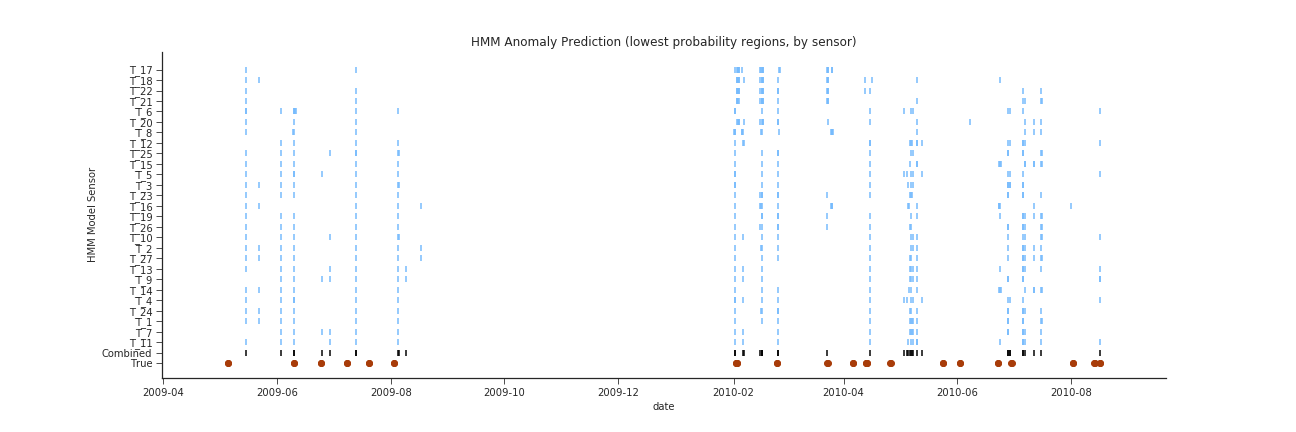
\includegraphics[width=\linewidth]{unsupervised.png}
    \caption{Markers indicate top-N predicted anomalies occurring at this time, where N is the true number of observed anomalies. }
    \label{fig:unsupervised}
\end{figure*}

\subsection{Supervised}
Use the probability features as input into a decision tree or SVM, instead of the original sensor data. We will do cross-validation, but making sure the "training" sets are always time-points \textit{before} the test sets. See how well that does? Fig.~\ref{fig:supervised} 

\begin{figure}
    \centering
    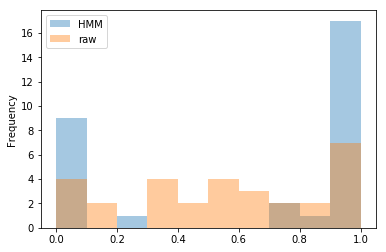
\includegraphics[width=\linewidth]{clf.png}
    \caption{Accuracy scores of Decision-tree model, over 30 time-series-splits used for cross-validation. }
    \label{fig:supervised}
\end{figure}
It does OK...more do well, but more do poorly too. This indicates there is some minimum amount of time the model needs before the probabilities are useful. This model either does great or terrible, while before it was a whole lot of mediocre. 

% \section{DEFINITION STUFF}
% I just put things you had into a section to be sorted later. 
% \subsection{Terms I don't know if we need anymore}

% \subsubsection{Support Vector Machine}\cite{SVM}
% The Support Vector Machine (SVM) is a commonly used binary-classification tool. A pure, hard-margin SVM is ideal for data that is linearly separable. However we didn't really use this, did we?

% \subsubsection{Singular Value Decomposition}
% Singular Value Decomposition (SVD) is a method of data dimensional reduction. It's useful, but I don't know how relevant it's going to be if we use the ``swinging door" compression thing.

% \subsubsection{Principle Component Analysis}
% Did we use this for anything other than justification? Is it worth talking about anymore?

% \subsection{K means clustering}\label{sec:kmeans}
% K-Means Clustering is a useful tool for classifying unlabeled data based. Classification is based upon a user-selected number of clusters ``K" data will be classified into. The number of clusters ``K" is associated with the number of visible \textbf{symbols/states}\footnote{from here on ``symbols" will be used}. Simple classification, first discussed by Lloyd, is based upon constant optimization of cluster centroids \cite{pcm} . Unfortunately, this makes K-Means susceptible to noise. For the purposes of this investigation, K-Means Clustering is implemented when using both Gaussian Mixture Models (Section \ref{sec:gmm}) as well as Hidden Markov Models (Section ~\ref{sec:hmm}).

% \subsection{Gaussian Mixture Model}\label{sec:gmm}
% When working with functions such as Fig. (normalized temperature density), it can be useful to interpret them as the sum of Multiple Gaussian distributions. The generated Gaussian components of the function are referred to as ``modes". Mode density must be selected carefully, as too few will result in under-fitting, whereas too many will over-fit the sum. To preclude this, components can be be dynamically added or removed depending upon their relevance to updating data \cite{GMM}.

% The number of modes in a function can be considered the number of visible symbols, and is used as the ``K" value as discussed in Section \ref{sec:kmeans}. Creation of discrete modes is shown to be an effective means of separating data by Zivkovic through image processing applications \cite{GMM}.
% Computing the appropriate number of visible symbols will be discussed in Section.

% \subsection{Hidden Markov Model}\label{sec:hmm}



\bibliographystyle{plainnat}
\bibliography{biblio}
\end{document}
